\chapter{Oracle APEX}

\section{Pengertian Oracle APEX}
Oracle Apex (Application Express) merupakan sebuah Aplikasi database berbasis web yang digunakan dalam database Oracle. Oracle Apex ini hanya menggunakan web browser saja dan proses pemrograman yang sederhana, serta mengembangkan ilmu dan kemampuan dengan Aplikasi ini aman dan cepat. Aplikasi Oracle Apex ini memiliki kualitas database yang bagus, produktifitas dan standart luas yang dimiliki oleh perusahaan – perusahaan besar dan memiliki keamanan, stabilitas, ketersediaan dalam membangun suatu web. Aplikasi ini merupakan suatu alat yang digunakan untuk membangun Aplikasi web- Based. Selain itu Oracle Apex tidak membutuhkan perangkat lainnya untuk mengembangkan, menyebarkan, serta menjalankan aplikasi, karena di dalam Oracle Apex ini telah menyediakan tiga alat utama seperti : 
\begin{enumerate}
    \item Application Builder : Yang digunakan untuk membuat aplikasi, melihat aplikasi, mengimport aplikasi, mengatur service, mengatur user aplikasi dan memantau aktifitas yang dilakukan pengguna.
    \item SQL Workshop : Yang digunakan untum membuat table dan komponennya (menggnakan kode PL – SQL secara manual maupun otomatis), melihat struktur table dan komponennya, mengimpor dan mengekspor script.
    \item Utilitas : Yang digunakan untuk melihat report table dan komponennya serta history aplikasi.
\end{enumerate}

\section{Pengembangan Aplikasi di Perusahaan}
\begin{enumerate}
    \item membutuhkan sumber daya pengembangan khusus dan mahal
    \item siklus dev aplikasi lama
    \item tumpukan besar
    \item kolaborasi minimal
    \item bisnis memecahkan masalah dengan alat yang salah
\end{enumerate}

\section{Mengelola data spreadsheet}
  \begin{enumerate}
      \item Validasi data    -- manual dan rawan error
      \item Integritas data  -- tidak menjamin keakuratan data dalam lingkungan multiuser
      \item Keamanan data    -- penguncian sel tidak efektif
      \item Berbagi data     -- exel lamban dan sulit utuk dibagikan
  \end{enumerate}  
  
\section{Mengubah spreadsheet menjadi aplikasi web}
  \begin{enumerate}
      \item Sign in apex.oracle.com
      \item Membuat workspace
      \item Buka app builder >create a new app>  drag dan drop file> pilih movie > next
      \item isi pada table nama, serta jenis huruf yang digunakan
      \item setelah itu create application lalu akan memasuki appreance yang dimana berisikan jenis- jenis tabel yang ada, pilih icon sesuai keinginan. pada feature centang semua kolom
      \item run aplikasi dengan memasukan kata sandi dan username
\end{enumerate}


\section{Aplikasi Yang Cocok Untuk Oracle Apex}
\begin{enumerate}
\item aplikasi mission-critical besar untuk ribuan pengguna
\item mengisi kekosongan dalam sistem perusahaan
\item merampingkan proses bisnis yang sudah ketinggalan zaman
\item modernisasi sistem warisan
\item aplikasi layanan mandiri untuk semua karyawan
\item portal yang menghadap pelanggan / mitra
\item aplikasi responsif yang berfungsi pada perangkat apa pun
\item bukti konsep
\item aplikasi quick-win (umur <beberapa monhts)
\item mengganti spreadsheet
\end{enumerate}


    
\section{Cara Membuat Tabel HR}
\begin{enumerate}
    \item Buka Oracle Apex
    \item Jika sudah masuk, pilih Object Browser>Create >Table
    \item Tentukan nama table dan nama skema yang menjadi milik table baru pada klausa CREATE TABLE.
    \item Setelah itu daftarkan semua kolom table di dalam tanda kurung. Jika sebuah table memiliki beberapa kolom, maka harus dipisahkan dengan koma (,). Definisi kolom mencakup nama kolom diikuti oleh tipe datanya, missal Number, Varchar2, dan batasan kolom seperti Bukan Nul.
    \item Contoh : membuat sebuah table dengan nama “employee” pada database “hris” dengan script berikut :
\begin{figure}[!htbp]
    \centering
    \includegraphics[scale=0.45]{section/tabel_hr.JPG}
\end{figure}
    \item Apabila keluar pesan “Query OK”, berarti anda telah sukses membuat table “employee”.
    \end{enumerate}

    
Penjelasan :
\begin{enumerate}
    \item able name adalah nama table yang telah anda buat. Setiap table didalam database harus unik, tidak boleh ada yang sama.
    \item Column name1, colum name2, column name3, dan seterusnya adalah nama kolom yang ditambahkan ke dalam table dimana data akan disimpan.
    \item Data type adalah tipe data yang disematkan pada kolom. Tipe data menentukan data yang boleh dimasukkan ke dalam kolom yang bersangkutan
    \item Not Null adalah salah satu jenis consistraint yang dapat anda berikan pada sebuah kolom. Consistraint ini bersifat optional, jika ditambahkan berarti kolom yang bersangkutan tidak boleh kosong (null)
    \item Auto Increment adalah salah satu opsi tambahan, apabila kolom yang bersangkutan akan dijadikan sebagai sequence, yaitu data yang akan dimasukkan otomatis bertambah satu
    \item Primary Key adalah salah satu jenis constraint, dimana kolom yang bersangkutan akan dijelaskan sebgai kunci primer di sebuah table. Tujuannya adalah menjaga integritas data.
\end{enumerate}



\section{Tahapan Membuat Aplikasi Oracle Apex}
Pertama kita buka websitenya yaitu https://apex.oracle.com, kita akan mendapatkan akses untuk memasuki Oracle Apllication Express, masukan email anda yang valid untuk membuat Workspace,  bagaimana tahapan pembuatan Aplikasi pada Oracle APEX :
\begin{enumerate}
    \item Pergi ke halaman website https://apex.oracle.com/

\begin{figure}[!htbp]
    \centering
    
\includegraphics[scale=0.4]{section/ica2.JPG}
    \label{gambar 1}
\end{figure}

    \item Klik Request a Free Worksace.
    
\begin{figure}[!htbp]
    \centering
    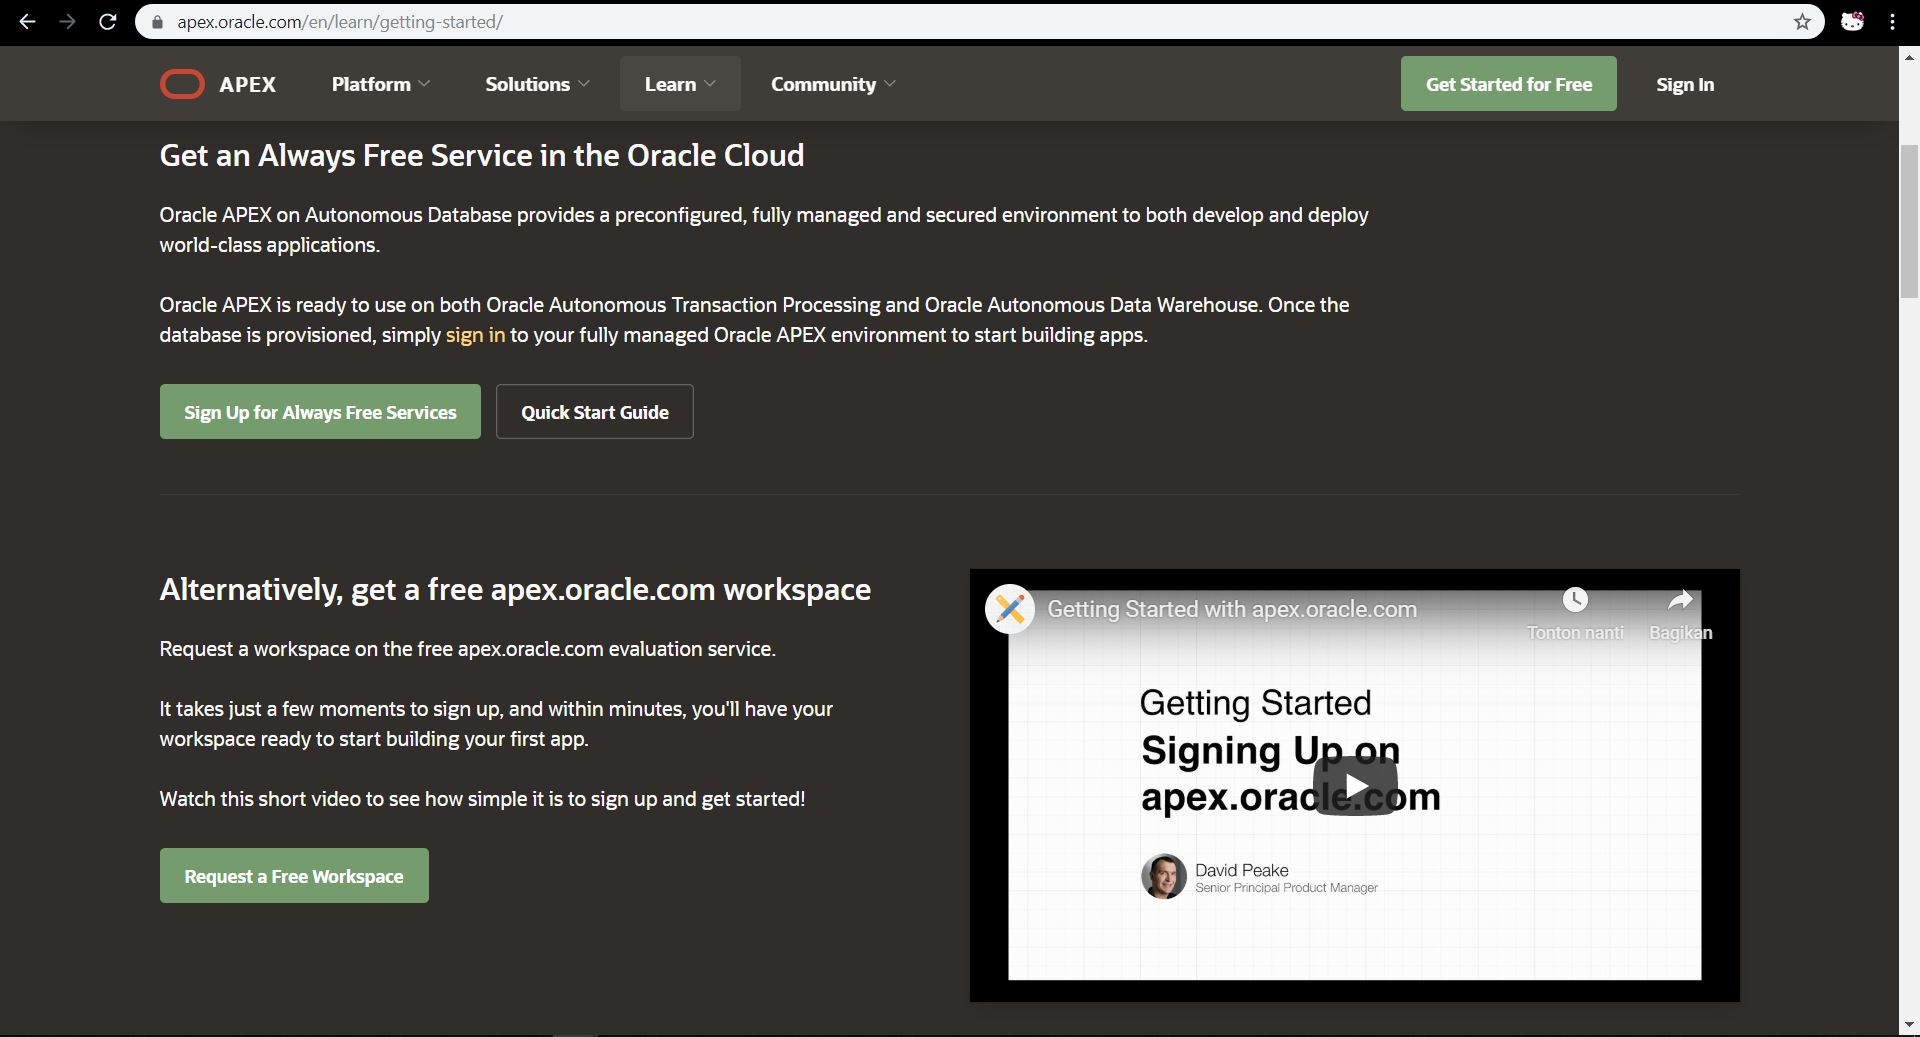
\includegraphics[scale=0.3]{section/ica3.JPG}
    \label{gambar 1}
\end{figure}
\vspace{3cm}
    \item Isikan data diri anda seperti nama,email,dan workspace.
    
    \begin{figure}[!htbp]
    \centering
    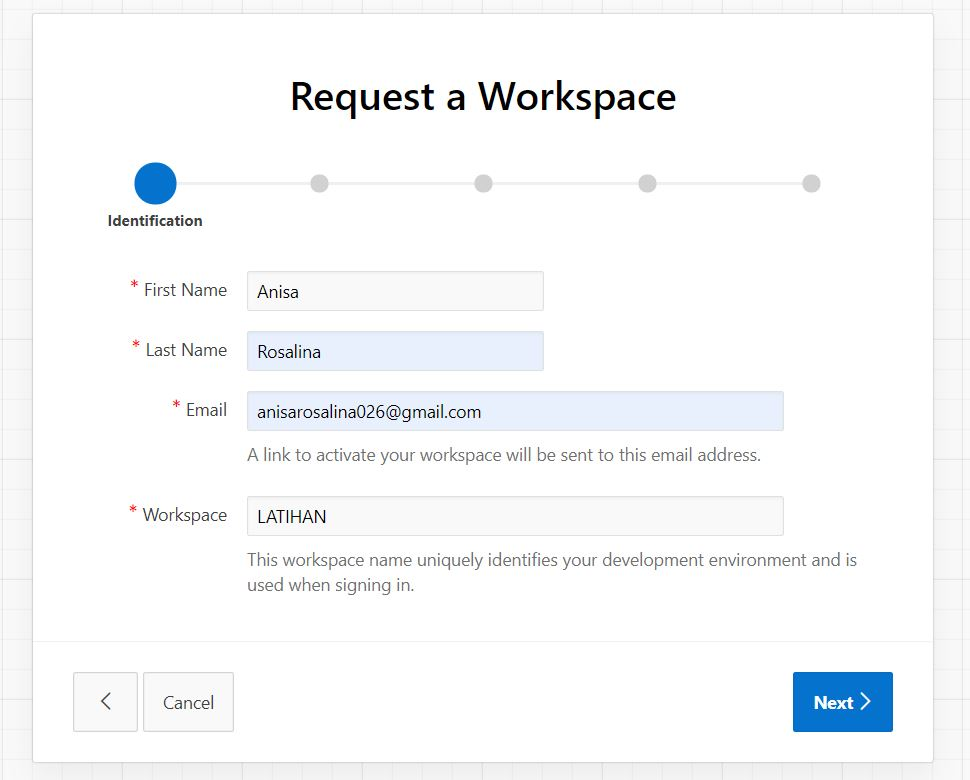
\includegraphics[scale=0.5]{section/ica4.JPG}
    \label{gambar 1}
\end{figure}

    \item Centang apakah anda pernah melakukan hal tersebut lalu next. 

    \begin{figure}[!htbp]
    \centering
    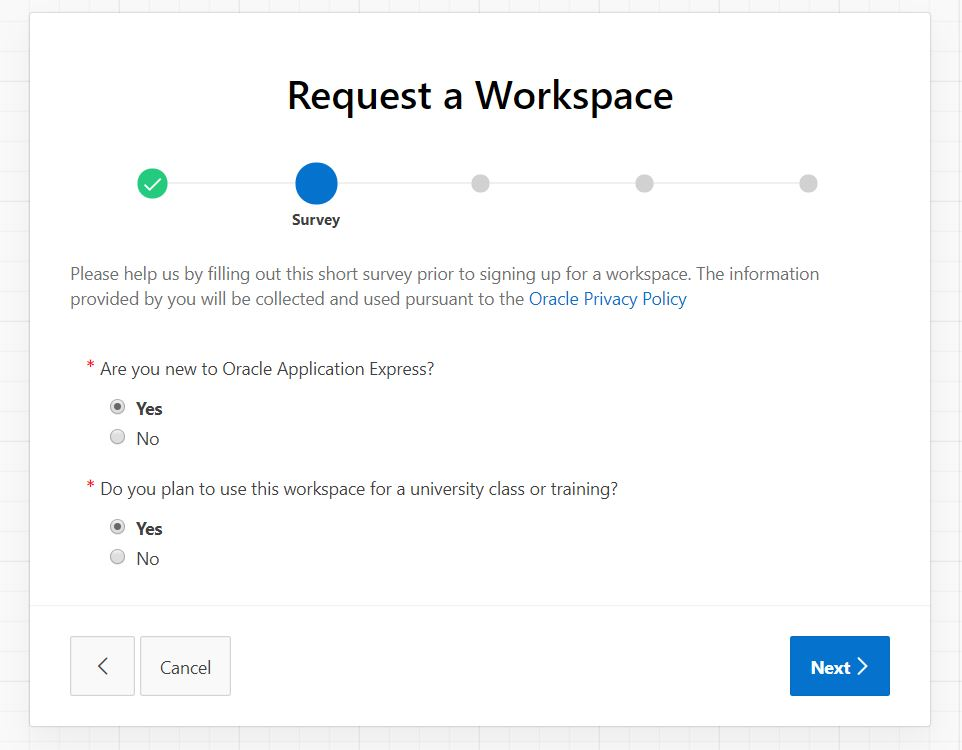
\includegraphics[scale=0.5]{section/ica5.JPG}
    \label{gambar 1}
\end{figure}
\vspace{6cm}
\item Isikan pada kolom tersebut bebas, mengapa anda ingin menggunakan layanan ini ?, lalu klik next.

    \begin{figure}[!htbp]
    \centering
    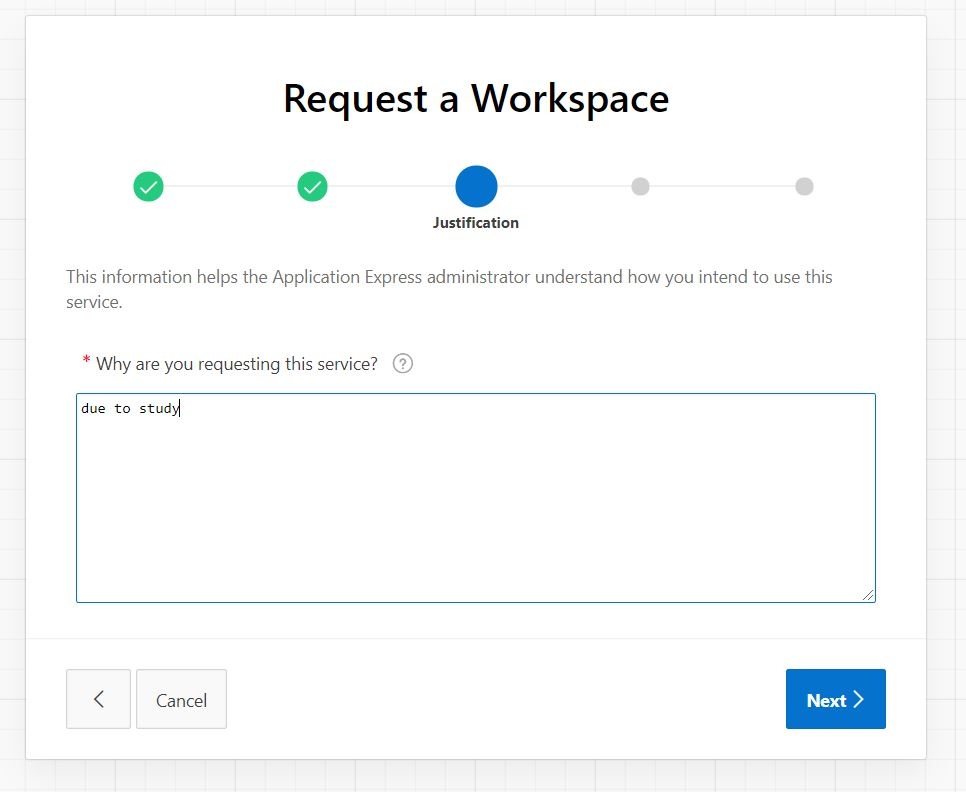
\includegraphics[scale=0.5]{section/ica6.JPG}
    \label{gambar 1}
\end{figure}

\item Centang Accept, lalu klik next.

   \begin{figure}[!htbp]
    \centering
    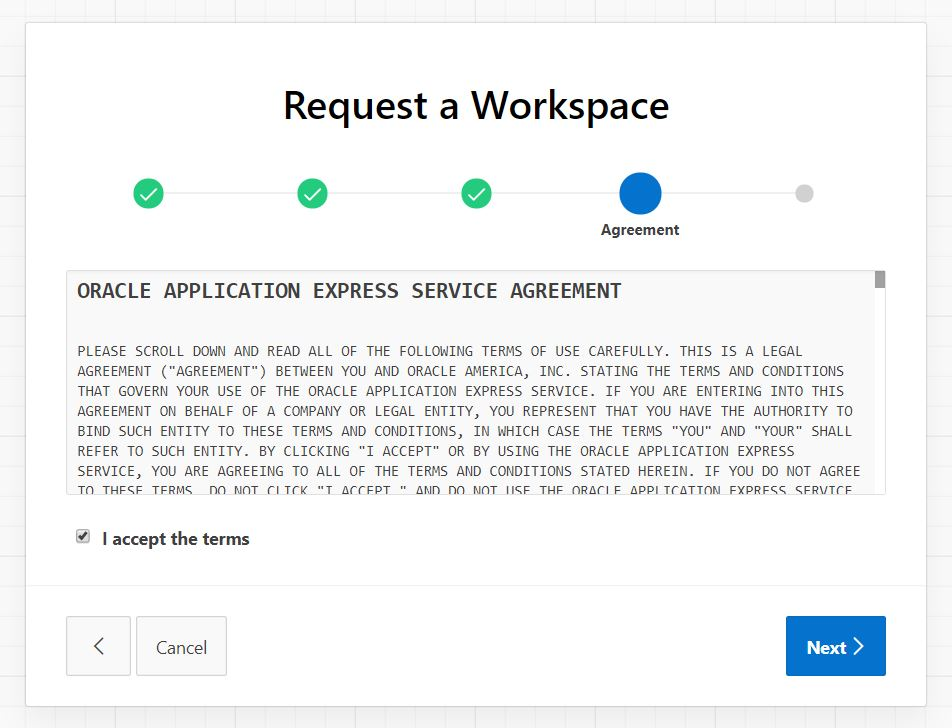
\includegraphics[scale=0.5]{section/ica7.JPG}
    \label{gambar 1}
\end{figure}
\vspace{6cm}
\item Tahapan terakhir untuk mengkonfirmasi apakah ini anda, lalu klik next.

   \begin{figure}[!htbp]
    \centering
    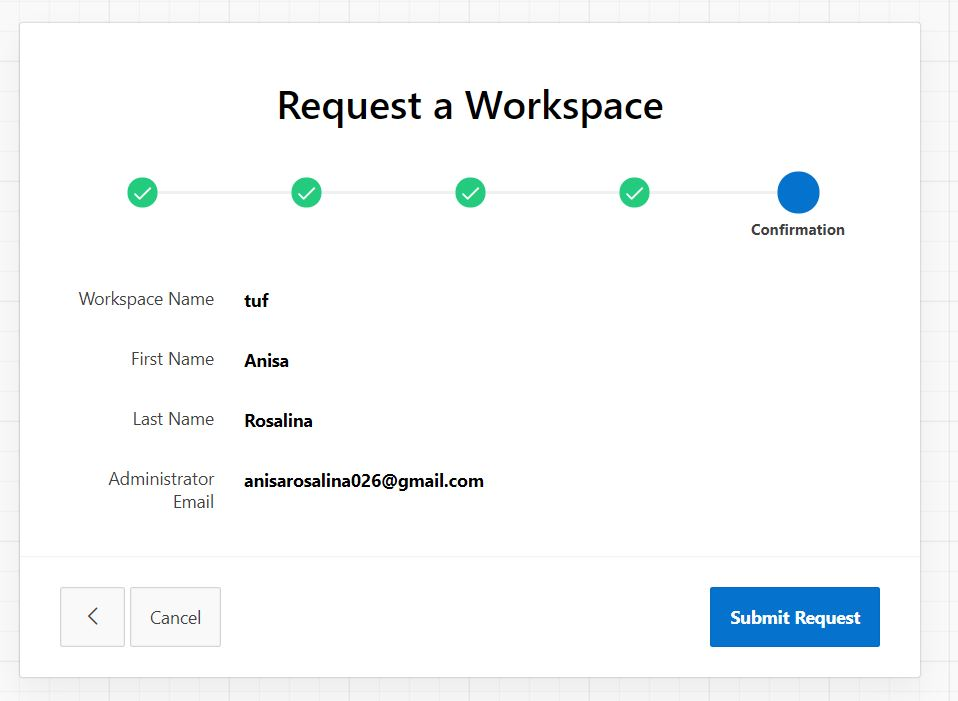
\includegraphics[scale=0.5]{section/ica8.JPG}
    \label{gambar 1}
\end{figure}

\item Finish, lalu lihat email anda.

   \begin{figure}[!htbp]
    \centering
    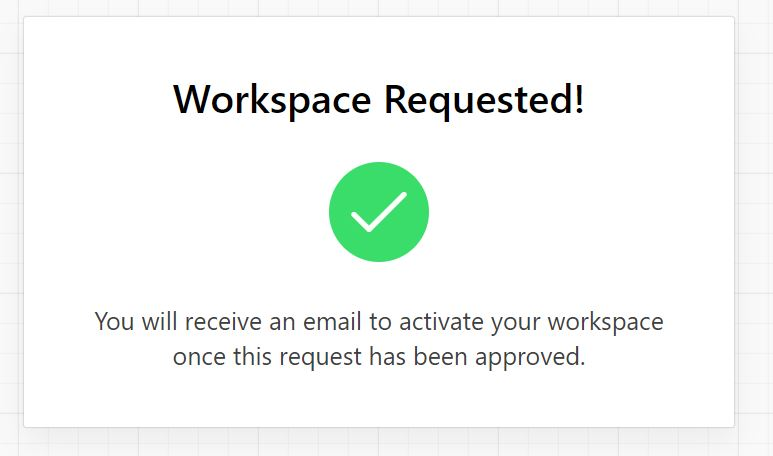
\includegraphics[scale=0.6]{section/ica9.JPG}
    \label{gambar 1}
\end{figure}

\vspace{8cm}

    \item Workspace anda telah di Acc lalu klik continue.
       \begin{figure}[!htbp]
    \centering
    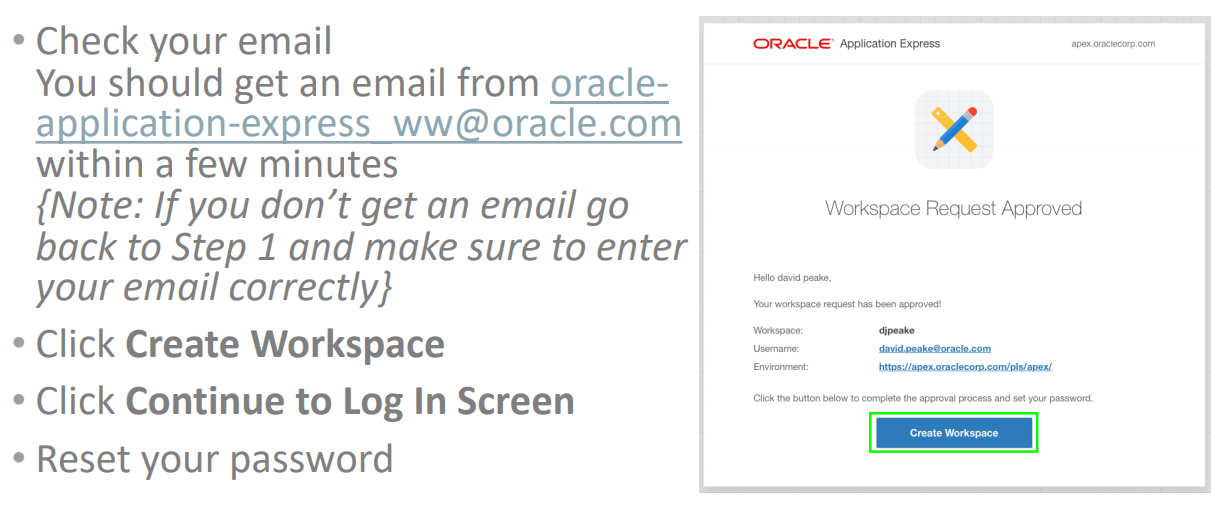
\includegraphics[scale=0.5]{section/ica10.PNG}
    \label{gambar 1}
\end{figure}
\item WorkspaceWorkspace kamu telah dibut lalu lanjutkan klik sign in.
       \begin{figure}[!htbp]
    \centering
    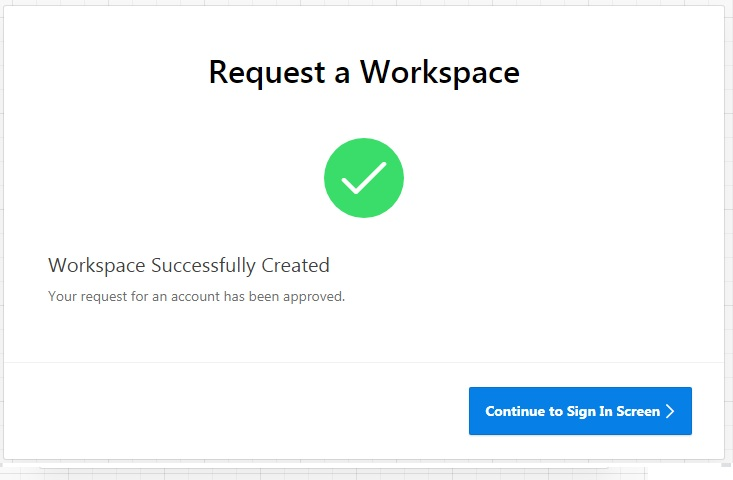
\includegraphics[scale=0.6]{section/ica12.jpg}
    \label{gambar 1}
\end{figure}
\vspace{12cm}

\vspace{4cm}








  \begin{enumerate}
   
      
  \end{enumerate}
  \end{enumerate}
